
\subsection{Task 2 (Targeted) vs Task 3 (Improved Targeted)}


\begin{solve}

The plots of purturbed images and the original images are shown below for both the tasks. The success rate and accuracy plots are also shown for both the models.

\textbf{Improved Targeted Attack}
For the improvement in the target attack, we follow the dicscussion from the recitation, where the TA said that LR decay, adptive techniques can be further used to improve the attack. However, we did not implement them.

In this version of improved attack, I implemeted the following updates to the PGD attack with Adam Momentum:
\begin{itemize}
    \item LR Decay was incorporated in the attack. The learning rate was decayed by a factor of 0.25 after every 10 iterations.
    \item Early Stopping was added in the attack. The attack was stopped if the loss was in the tolerance of $1e-3$ .
    \item Random Initialization was added to the attack. The attack was initialized with a random perturbation instead of always starting from the same perturbation.
    \item Lastly, an adaptive $\epsilon$ was used. The epsilon was increased by a factor of 1.2 after every 10 iterations.
\end{itemize}
% Note that in the case of targeted attacks, we used PGD. Given the value of $\alpha = .0392$, we see that the attack is quite visible even for $\epsilon \sim .04$


\textbf{Model A vs Model B for Targeted and Improved Targeted Attack}

\begin{itemize}
    \item For Targeted attacks, the success rate is higher for Model A than Model B. Infact we are unable to get any successful attack on Model B even with very high $\epsilon$ values as compared to Model A for the same $\alpha$ values.
    \item 
    We also see that the test accuracy does not change for model B during the attack, showing that not only we are failing in targeted attacks but we are also not able to misclassify the images in untargeted sense.
    This shows that Model B is more robust to attacks than Model A in this setting.

    \item We see the same is true for improved targeted attacks. The success rate is higher for Model A than Model B. Even for very high $epsilon$ values.
\end{itemize}


I have added the plots for other $\epsilon$ n the submission, but here are the plots for $\epsilon = 0.0980$ for both the models for both the attacks.

\begin{figure}[H]
    \centering
    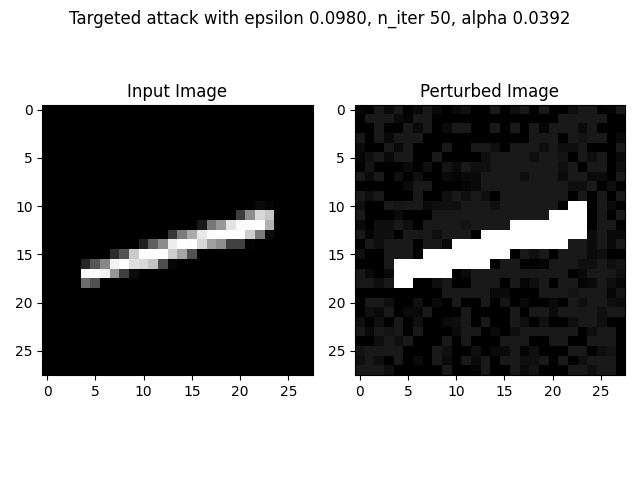
\includegraphics[trim={0 1.5cm 0cm 0}, width=.5\textwidth]{/Users/vashisth/Documents/GitHub/Intro_DL/IDL_HW3/HW3_tex/plots/Del6/Targeted/Targeted_attack__modA_e-0.0980_a-0.0392Img-2_iter50.png}
    \caption{Targeted Attack on Model A with $\epsilon = 0.0980$, $\alpha = 0.0392$, 50 iterations}
    \centering
    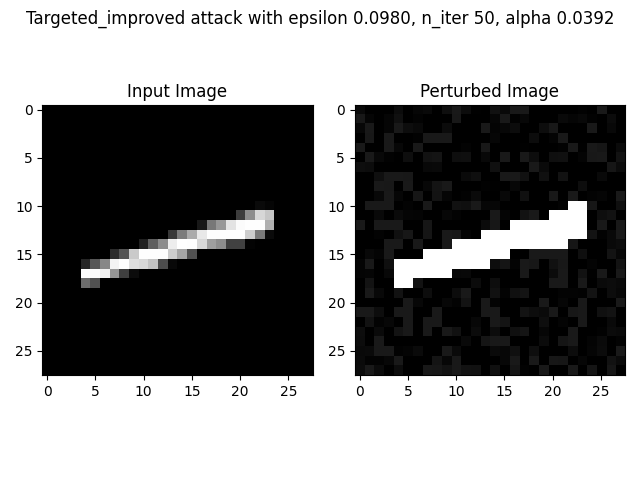
\includegraphics[trim={0 1.5cm 0cm 0}, width=.5\textwidth]{/Users/vashisth/Documents/GitHub/Intro_DL/IDL_HW3/HW3_tex/plots/Del6/Targeted_improved/Targeted_improved_attack__modA_e-0.0980_a-0.0392Img-2_iter50.png}
    \caption{Improved Targeted Attack on Model A with $\epsilon = 0.0980$, $\alpha = 0.0392$, 50 iterations}
\end{figure}
We see that the improved attack is a bit harder to detect.

\begin{figure}[H]
    \centering
    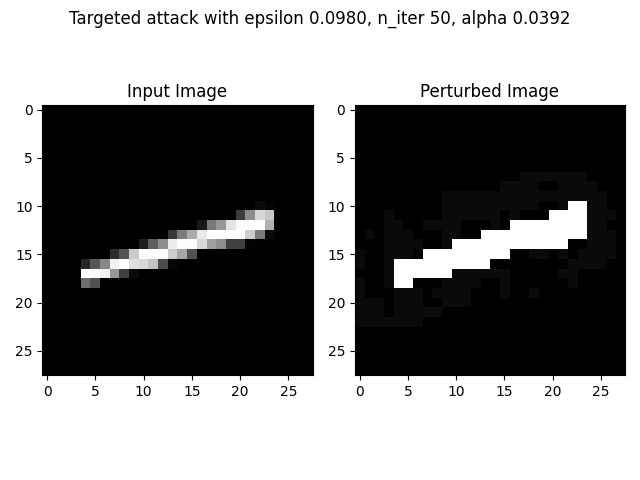
\includegraphics[trim={0 1.5cm 0cm 0}, width=.5\textwidth]{/Users/vashisth/Documents/GitHub/Intro_DL/IDL_HW3/HW3_tex/plots/Del6/Targeted/Targeted_attack__modB_e-0.0980_a-0.0392Img-2_iter50.png}
    \caption{Targeted Attack on Model A with $\epsilon = 0.0980$, $\alpha = 0.0392$, 50 iterations}
    \centering
    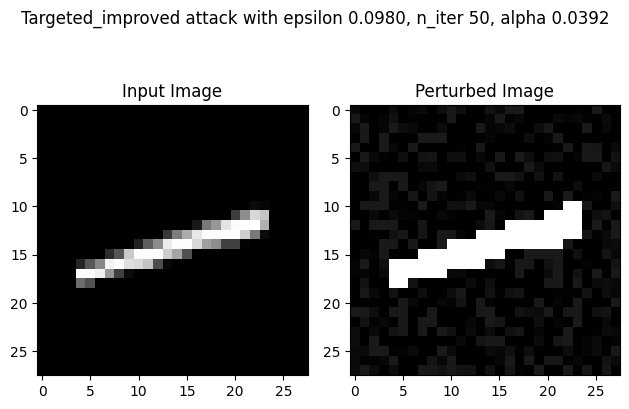
\includegraphics[trim={0 0cm 0cm 0}, width=.5\textwidth]{/Users/vashisth/Documents/GitHub/Intro_DL/IDL_HW3/HW3_tex/plots/Del6/Targeted_improved/modB-0.0980_a-0.0392Img-2_iter50.png}
    \caption{Improved Targeted Attack on Model B with $\epsilon = 0.0980$, $\alpha = 0.0392$, 50 iterations}
\end{figure}



\begin{figure}[H]
    \centering
    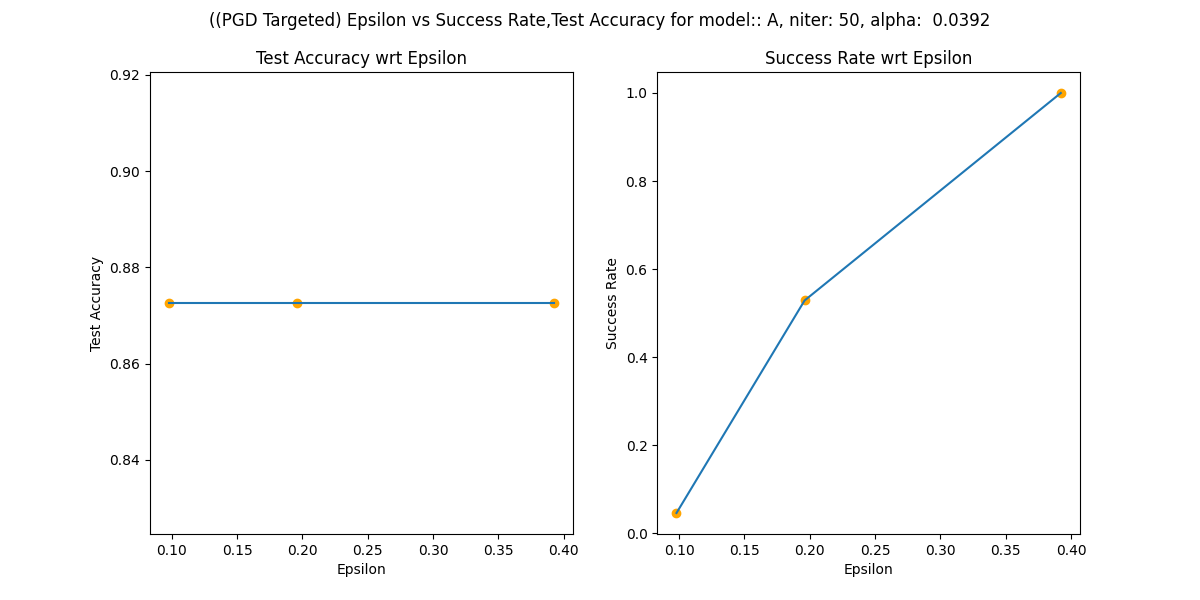
\includegraphics[width = .45 \textwidth]{/Users/vashisth/Documents/GitHub/Intro_DL/IDL_HW3/HW3_tex/plots/Del6/success_rate_plot_(PGD Targeted)_modA_iter50_a-0.0392.png}
    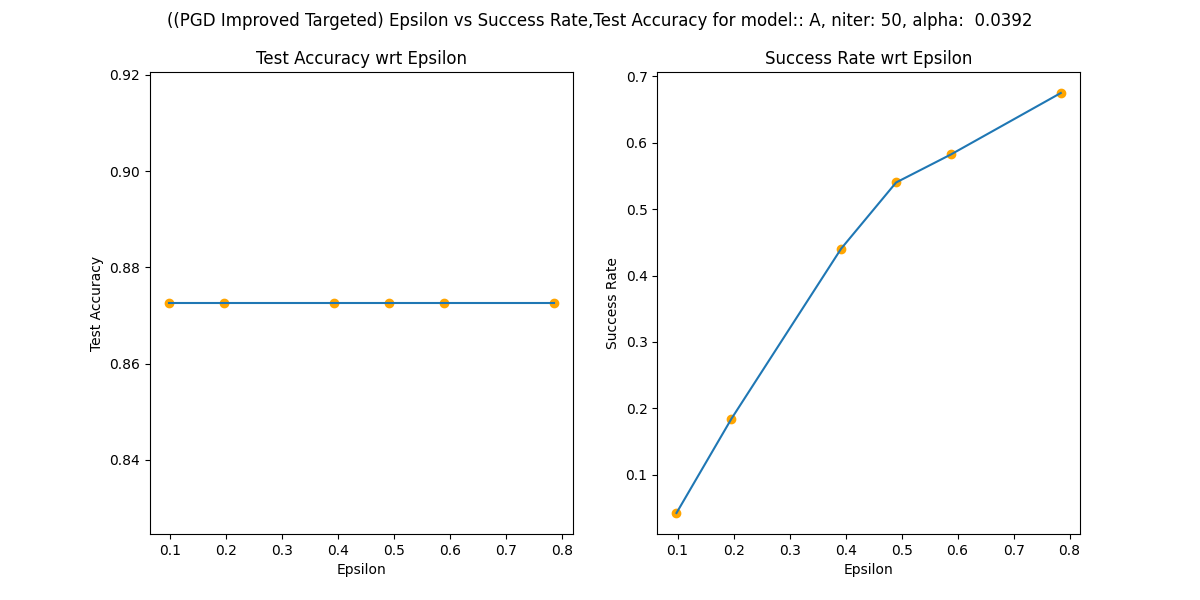
\includegraphics[width = .45 \textwidth]{/Users/vashisth/Documents/GitHub/Intro_DL/IDL_HW3/HW3_tex/plots/Del6/success_rate_plot_(PGD Improved Targeted)_modA_iter50_a-0.0392.png}
    \caption{Success Rate and Accuracy Plot for Targeted Attack vs Improved Targeted Attack on Model A}
%%%%%%%%%
    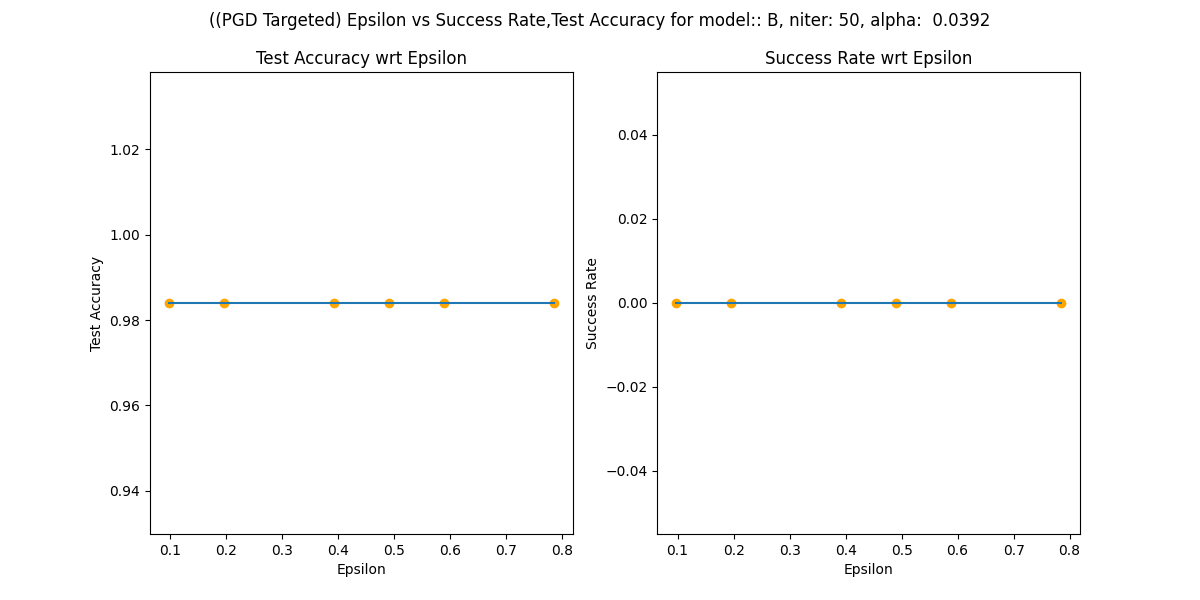
\includegraphics[width = .45 \textwidth]{/Users/vashisth/Documents/GitHub/Intro_DL/IDL_HW3/HW3_tex/plots/Del6/success_rate_plot_(PGD Targeted)_modB_iter50_a-0.0392.png}
    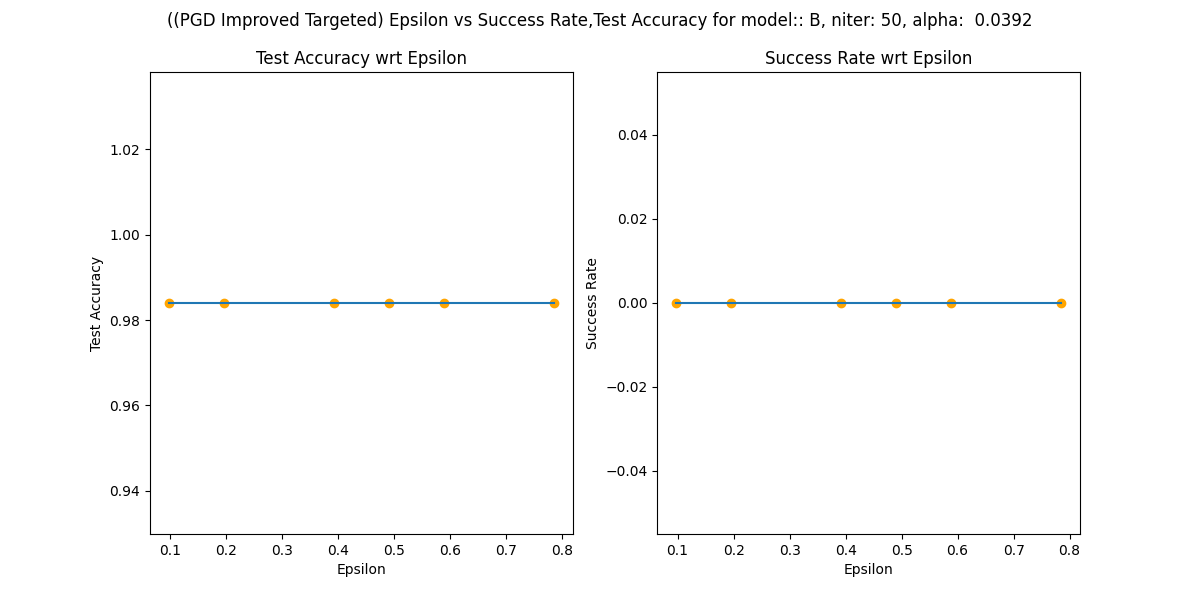
\includegraphics[width = .45 \textwidth]{/Users/vashisth/Documents/GitHub/Intro_DL/IDL_HW3/HW3_tex/plots/Del6/success_rate_plot_(PGD Improved Targeted)_modB_iter50_a-0.0392.png}
    \caption{Success Rate and Accuracy Plot for Targeted Attack vs Improved Targeted Attack on Model B}
    \end{figure}
    
Again we see that despite the improved attack Model B doesnt get attacked. The success rate is 0 for Model B. The success rate for Model A is lower (by aroud .2) which might be due to not having the right hyper-parameters for momentum 1 and 2, and other scaling/decay factors.

\end{solve}




%%%%%%% 
\subsection{Bonus Task}


\begin{solve}
    For this $\alpha =  50/255$ was fixed for both the attacks. The $\epsilon$ values were $8/255, 16/255$ for the plots below.

\begin{figure}[H]
    \centering
    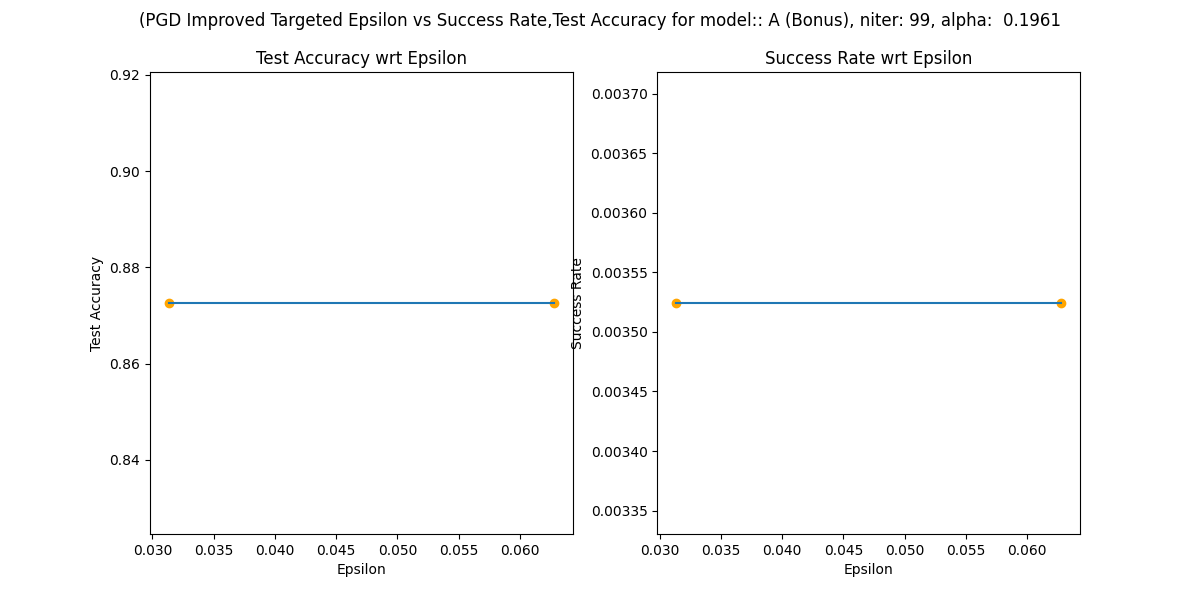
\includegraphics[width = .6 \textwidth]{/Users/vashisth/Documents/GitHub/Intro_DL/IDL_HW3/HW3_tex/plots/Del6/success_rate_plot_PGD Improved Targeted_modA (Bonus)_iter99_a-0.1961.png}

    \centering
    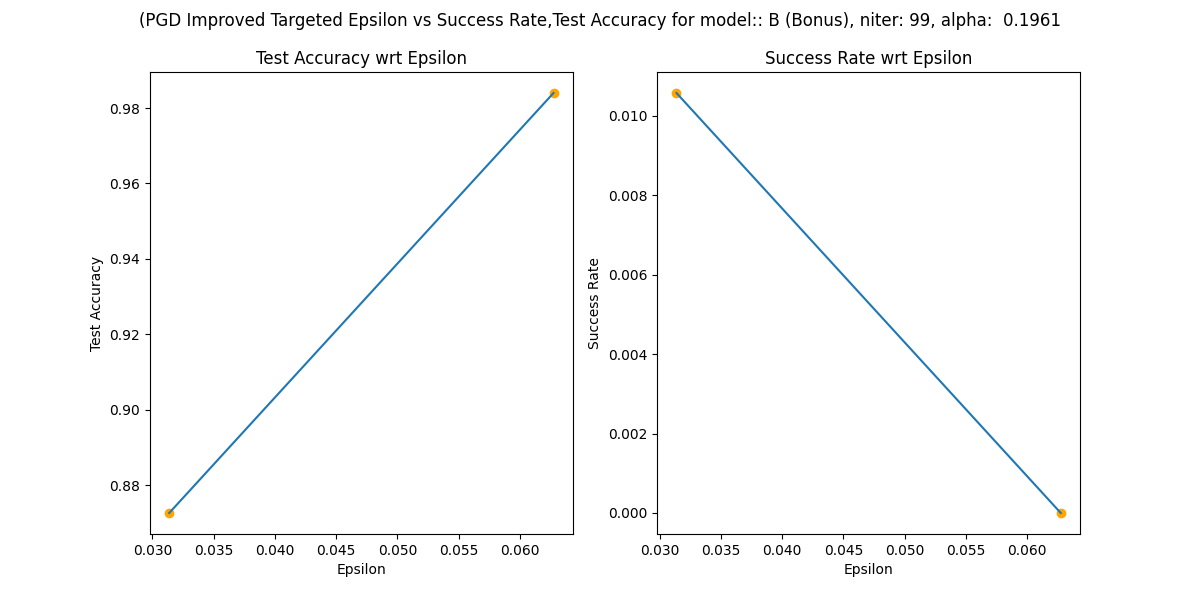
\includegraphics[width = .6 \textwidth]{//Users/vashisth/Documents/GitHub/Intro_DL/IDL_HW3/HW3_tex/plots/Del6/success_rate_plot_PGD Improved Targeted_modB (Bonus)_iter99_a-0.1961.png}

    \caption{Success Rate and Accuracy Plot for Improved Targeted Attack on Model A and B}
    \end{figure}

    For A we get a value of around $.00355$ for both $\epsilons$, for attack B we get success rate of $.010$ for smallest epsilon. I only got this for one run and got zero other runs. 

    Again showing Model B is very robust to the specific targeeted attack we are making in this case.
\end{solve}
